\subsection*{Question 2.11}

As seen in figure \ref{fig:q211.1} through \ref{fig:q211.3}, the
penalization parameter controls how much the green points are weighed
compared to the blue ones.

\begin{figure}[!htbp]
  \centering
  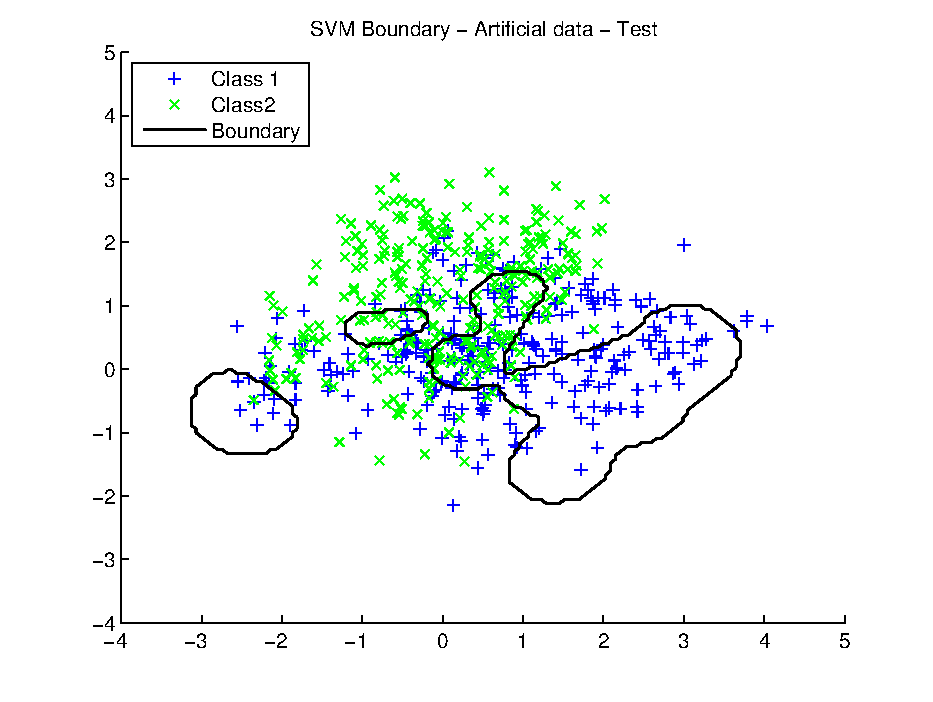
\includegraphics[width=0.6\textwidth]{./images/q211_0_1.pdf}
  \caption{Boundary when the penalization parameter is set to $0.1$.}
  \label{fig:q211.1}
\end{figure}
\begin{figure}[!htbp]
  \centering
  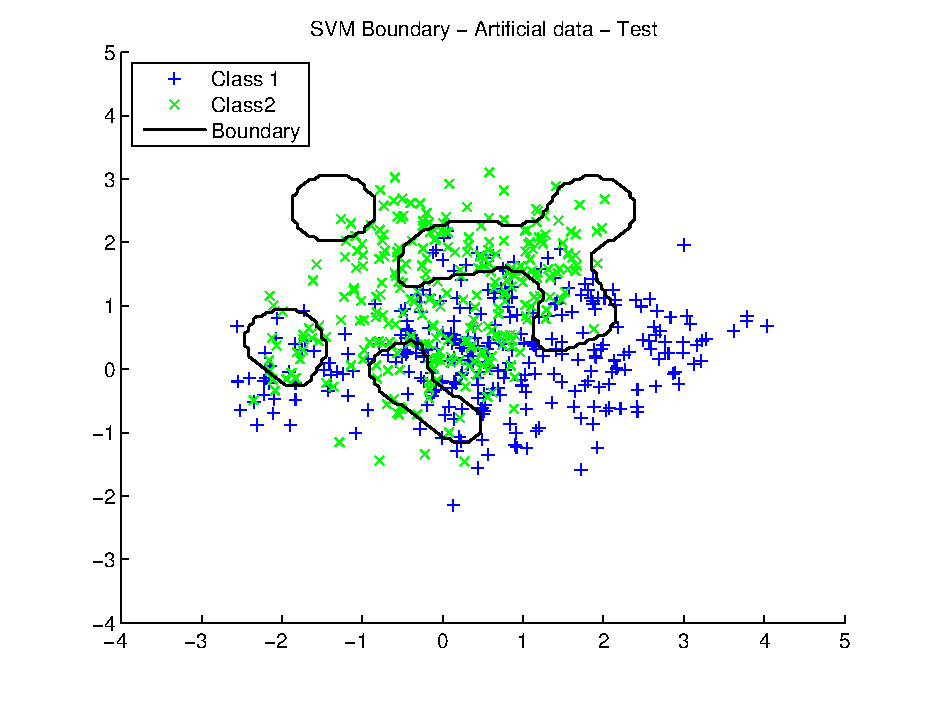
\includegraphics[width=0.6\textwidth]{./images/q211_01.pdf}
  \caption{Boundary when the penalization parameter is set to $1$.}
  \label{fig:q211.2}
\end{figure}
\begin{figure}[!htbp]
  \centering
  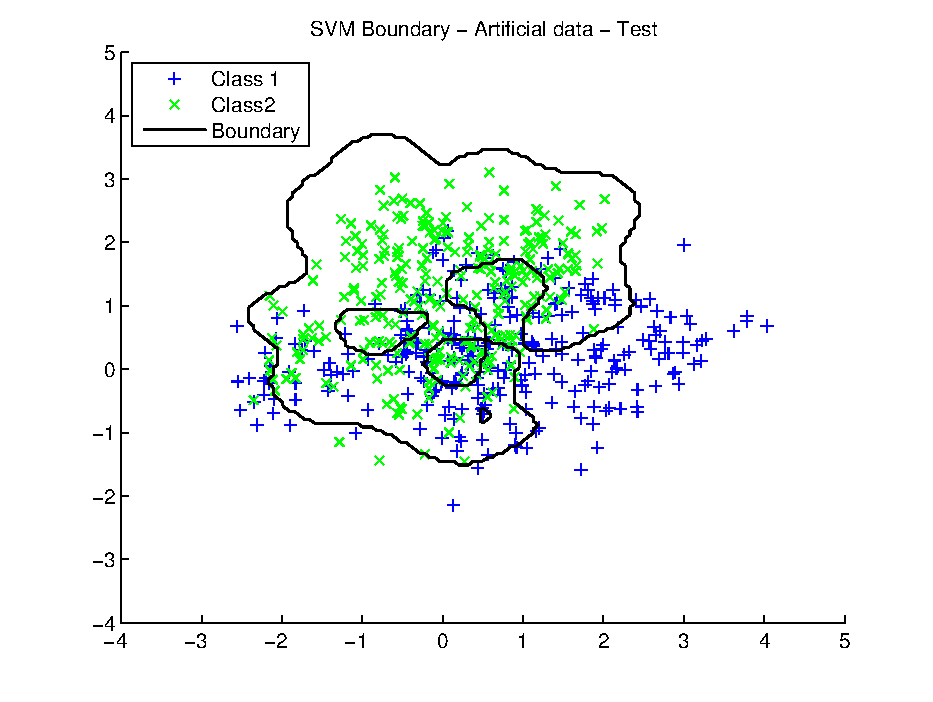
\includegraphics[width=0.6\textwidth]{./images/q211_10.pdf}
  \caption{Boundary when the penalization parameter is set to $10$.}
  \label{fig:q211.3}
\end{figure}

The general trend of the error as a function of the penalization
parameter can be seen in figure \ref{fig:q211.4}.  When variating the
length scale of the kernel function, the error variates as seen in
figure \ref{fig:q211.5}.

\begin{figure}[!htbp]
  \centering
  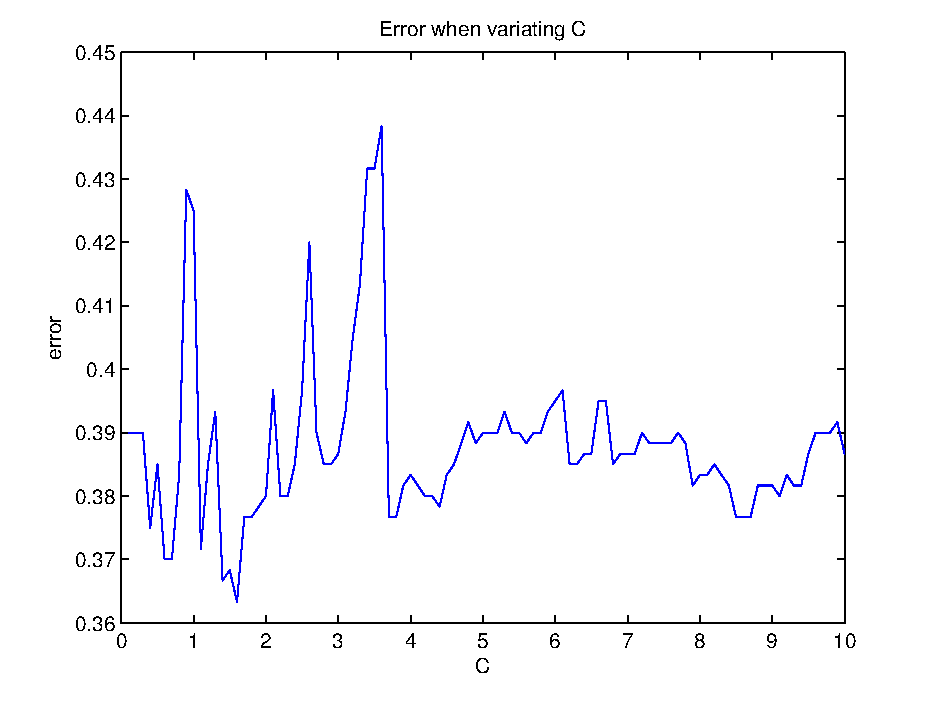
\includegraphics[width=0.6\textwidth]{./images/q211_errors.pdf}
  \caption{Error when variating the penalization parameter.}
  \label{fig:q211.4}
\end{figure}
\begin{figure}[!htbp]
  \centering
  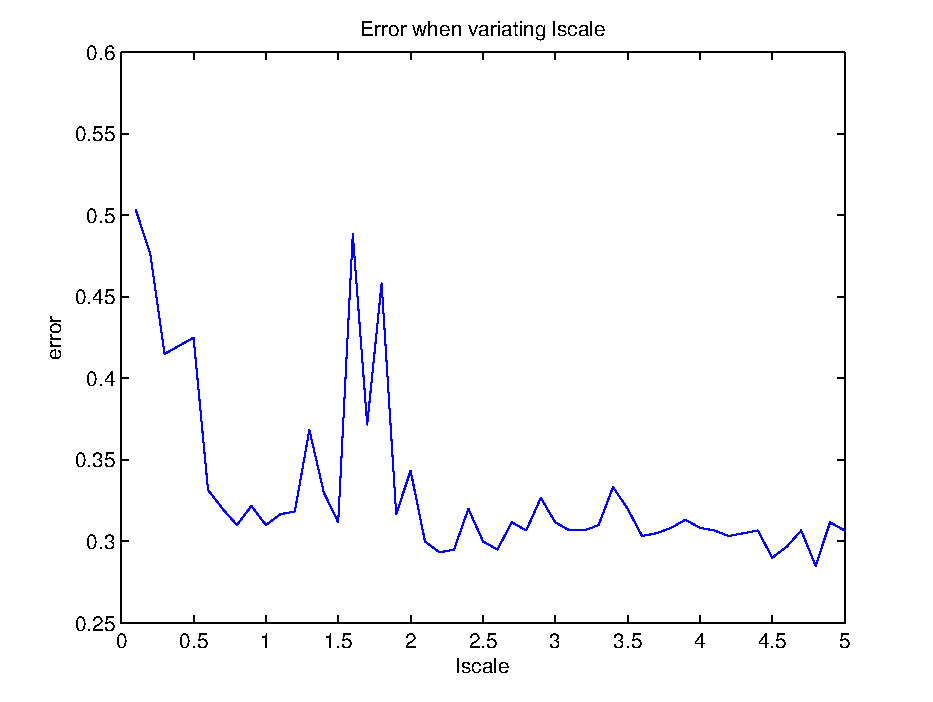
\includegraphics[width=0.6\textwidth]{./images/q211_errors_lscale.pdf}
  \caption{Error when variating the length scale of the kernel function.}
  \label{fig:q211.5}
\end{figure}
